\documentclass[14pt]{extarticle}
\usepackage[spanish]{babel}
\usepackage[utf8]{inputenc}
\usepackage{enumerate}
\usepackage{xparse, amsmath, physics,graphicx}
\usepackage{cancel}

\decimalpoint

\usepackage{anysize}
\marginsize{1cm}{1cm}{1.3cm}{1.3cm}
\renewcommand{\baselinestretch}{1.2}
\parindent  = 0mm
\parskip = 4mm

\usepackage[usenames]{color}
\definecolor{azul}{RGB}{10,80,190}
\definecolor{negro}{RGB}{0,0,0}
\definecolor{rojo}{RGB}{190,80,10}
\definecolor{verde}{RGB}{0,120,50}

\begin{document}
    \title{
        Matemáticas para las ciencias aplicadas IV\\
        Tarea 1
    }
    \author{
        Careaga Carrillo Juan Manuel\\
        Quiróz Castañeda Edgar\\
        Soto Corderi Sandra del Mar
    }
    \date{13 de marzo de 2019}
    \maketitle
    \thispagestyle{empty}
    \pagebreak
    \begin{enumerate}
        % Ejercicio 1
        \item {
            Resolver las ecuaciones diferenciales
            \begin{enumerate}
                % a)
                \item {
                    $t(t-4)\frac{dy}{dt} + y = 0$
                    con $y(2)=1$

                    \color{azul}
                    % Respuesta
                     Modificando la ecuación, tenemos que
                    \begin{align*}
                    &\implies \dv{y}{t} = \frac{-1}{t(t-4)}y
                    \end{align*}
                    Que es de la forma de una ecuación lineal homogénea.\\[.3cm]

                    Por lo que, para resolverla, hay que resolver
                    \begin{align*}
                    y&= 1 \cdot e ^{\int _{2}^{t} \frac{1}{s(s-4)}ds} \\[.3cm]
                  	&= e ^{-\int _{2}^{t} \frac{1}{s(s-4)}ds}\\[.3cm]
                  	&\int _{2}^{t} \frac{1}{s(s-4)} ds = \int _{2}^{t} (\frac{a_{0}}{s} + \frac{a_{1}}{s-4})ds\\[.3cm]
                  	&\int _{2}^{t} \frac{1}{s(s-4)} ds = \int _{2}^{t} (\frac{a_{0} (s-4)}{s} + \frac{a_{1}(s)}{s-4})ds\\[.3cm]
                  	&a_{0} = -\frac{1}{4} a_{1} = \frac{1}{4}\\[.3cm]
                  	&\int _{2}^{t} \frac{1}{s(s-4)} ds = \int _{2}^{t} (-\frac{1}{4s} + \frac{1}{4(s-4)})ds\\[.3cm]
                  	& \int _{2}^{t} \frac{1}{s(s-4)} ds = -\frac{1}{4} ln|s| \Big|_{2}^{t} + \frac{1}{4} ln|s-4| \Big|_{2}^{t}\\[.3cm]
                  	& \int _{2}^{t} \frac{1}{s(s-4)} ds = -\frac{1}{4} ln|t| + \frac{1}{4} ln|2| + \frac{1}{4} ln|t-4| -\frac{1}{4} ln|2|\\[.3cm]
                  	& \int _{2}^{t} \frac{1}{s(s-4)} ds = -\frac{1}{4} (ln|t| - ln|t-4|)\\[.3cm]
                  	& = e^{\frac{1}{4} (ln|t| - ln|t-4|) }\\[.3cm]
                  	& = e^{\frac{1}{4} ln(|\frac{t}{t-4}|) }
                    \end{align*}

                   De ahí $y = e^{\frac{1}{4} ln(|\frac{t}{t-4}|)}$
                }

                % b)
                \item {
                    $\dv{y}{t}+\frac{t}{1+ t^2}y=1-\frac{t^3}{1+t^4}y$.
                    Graficar algunas soluciones.

                    \color{azul}
                    % Respuesta
                    Modificando la ecuación, tenemos que
                    \begin{align*}
                    &\implies \dv{y}{t} = 1 - (\frac{t^3}{1 + t^4} + \frac{t}{1 + t^2})y\\[.3cm]
                    &\implies \dv{y}{t} + (\frac{t^3}{1 + t^4} + \frac{t}{1 + t^2})y = 1
                    \end{align*}
                    Que es de la forma de una ecuación lineal no homogénea.\\[.3cm]
                    Por lo que, para resolverla, hay que resolver
                    \begin{align*}
                    y&= \frac{1}{\mu} (\int \mu\cdot 1 dt + C)\\[.3cm]
                    &\mu = e^{\int (\frac{t^3}{1 + t^4} + \frac{t}{1 + t^2})dt}\\[.3cm]
                    &\int (\frac{t^3}{1 + t^4} + \frac{t}{1 + t^2})dt = \frac{1}{4} ln|1 + t^4| + \frac{1}{2}ln|1+t^2|\\[.3cm]
                    &\mu = e^{\frac{1}{4} ln|1 + t^4| + \frac{1}{2}ln|1+t^2|}\\[.3cm]
                    &\mu = e^{\frac{1}{4} ln|1 + t^4|} e^{\frac{1}{2}ln|1+t^2|}\\[.3cm]
                    &\mu = (e^{ln|1 + t^4|})^{\frac{1}{4}} (e^{ln|1+t^2|})^{\frac{1}{2}}\\[.3cm]
                    &\mu = (1 + t^4)^{\frac{1}{4}}(1+t^2)^{\frac{1}{2}}\\[.3cm]
                    y&= \frac{1}{(1 + t^4)^{\frac{1}{4}}(1+t^2)^{\frac{1}{2}}} (\int ((1 + t^4)^{\frac{1}{4}}(1+t^2)^{\frac{1}{2}} )dt + C)
                    \end{align*}

                    De ahí $y = \frac{\int ((1 + t^4)^{\frac{1}{4}}(1+t^2)^{\frac{1}{2}})dt + C}{(1 + t^4)^{\frac{1}{4}}(1+t^2)^{\frac{1}{2}}}$\\[.3cm]

                    La integral $\int ((1 + t^4)^{\frac{1}{4}}(1+t^2)^{\frac{1}{2}})dt$ no tiene una solución adecuada, así que utilizaremos el método de Euler con unos 10 valores para aproximar su gráfica.\\

                    La fórmula de Euler es:

                    $y_{k+1} = y_{k} + h[1 - (\frac{(t_{k})^3}{1 + (t_{k})^4} + \frac{t_{k}}{1 + (t_{k})^2})y_{k}]$, $k = 0,1,...,10$, $h = \frac{1}{10}$\\

                    Demos el valor $y_{0} = 0$ , $t_{0} = 0$\\

                    Tenemos que:
                    \begin{align*}
                    y_{1}&= 0 + 0.1[1- (\frac{0^3}{1+ 0^4} + \frac{0}{1+ 0^2} ) 0] = 0.1\\
                    y_{2}&= 0.1 + 0.1[1- (\frac{0.1^3}{1+ 0.1^4} + \frac{0.1}{1+ 0.1^2} ) 0.1] = 0.199\\
                    y_{3}&= 0.199 + 0.1[1- (\frac{0.2^3}{1+ 0.2^4} + \frac{0.2}{1+ 0.2^2} ) 0.199] = 0.295\\
                    y_{4}&= 0.295. + 0.1[1- (\frac{0.3^3}{1+ 0.3^4} + \frac{0.3}{1+ 0.3^2} ) 0.295] = 0.386\\
                    y_{5}&= 0.386 + 0.1[1- (\frac{0.4^3}{1+ 0.4^4} + \frac{0.4}{1+ 0.4^2} ) 0.386] = 0.470\\
                    y_{6}&= 0.470 + 0.1[1- (\frac{0.5^3}{1+ 0.5^4} + \frac{0.5}{1+ 0.5^2} ) 0.470] = 0.546\\
                    y_{7}&= 0.546 + 0.1[1- (\frac{0.6^3}{1+ 0.6^4} + \frac{0.6}{1+ 0.6^2} ) 0.546] = 0.611\\
                    y_{8}&= 0.611 + 0.1[1- (\frac{0.7^3}{1+ 0.7^4} + \frac{0.7}{1+ 0.7^2} ) 0.611] = 0.665\\
                    y_{9}&= 0.665 + 0.1[1- (\frac{0.8^3}{1+ 0.8^4} + \frac{0.8}{1+ 0.8^2} ) 0.665] = 0.709\\
                    y_{10}&= 0.709 + 0.1[1- (\frac{0.9^3}{1+ 0.9^4} + \frac{0.9}{1+ 0.9^2} ) 0.709] = 0.742
                    \end{align*}
                    
                    La gráfica se vería así:\\
                    
                    \centering
                    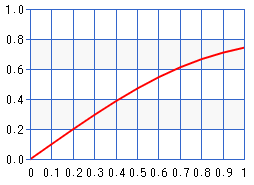
\includegraphics[width=10cm]{1b.png}\\
                    
                }

                % c)
                \item {
                    $\cos{y}\dv{y}{t}=\frac{-t\sin{y}}{1+t^2}$
                    con $y(1)=\frac{\pi}{2}$

                    \color{azul}
                    % Respuesta
                    Modificando la ecuación, tenemos que
                    \begin{align*}
                    &\implies \frac{\cos(y)}{\sin(y)}\dv{y}{t} = \frac{-t}{1 + t^2}\\[.3cm]
                    &\implies \dv{y}{t} = \frac{\frac{-t}{1 + t^2}}{ \frac{\cos(y)}{\sin(y)}}
                    \end{align*}
                    
                    Que es de la forma de una ecuación separable, donde $g(t) = \frac{-t}{1 + t^2}$ y $f(y) = \frac{\cos(y)}{\sin(y)}$.\\[.3cm]
                    
                    Por lo que, para resolverla, hay que resolver\\[.3cm]
                    
                    \begin{align*}
                    \int_{\frac{\pi}{2}}^{y} \frac{\cos(r)}{\sin(r)} dr &= \int_{1}^{t} \frac{-s}{1 + s^2} ds\\[.3cm]
                    ln|\sin(y)|\Big|_{\frac{\pi}{2}}^{y} &= -\frac{1}{2} ln|1 + s^2|\Big|_{1}^{t}\\[.3cm]
                    ln|\sin(y)| - ln|\sin(\frac{\pi}{2})| &= -\frac{1}{2} (ln|1 + t^2| - ln|1 + 1^2|)\\[.3cm]
                    ln|\sin(y)| &= -\frac{1}{2} (ln(|\frac{1 + t^2}{2}|)\\[.3cm]
                    \sin(y) &= (\frac{1 + t^2}{2})^{-\frac{1}{2}}\\[.3cm]
                    y &= \sin^{-1} (\sqrt{\frac{2}{1 + t^2}})
                    \end{align*}

                    De ahí $y = \sin^{-1} (\sqrt{\frac{2}{1 + t^2}})$\\[3.5cm]
                }

                % d)
                \item {
                    $\dv{y}{t}=1-t+y^2-ty^2$.
                    Graficar algunas soluciones.

                    \color{azul}
                    % Respuesta
                     Modificando la ecuación, tenemos que
                    \begin{align*}
                    &\implies \dv{y}{t} = (1-t) + y^2(1-t)\\[.3cm]
                    &\implies \dv{y}{t} = (1-t)(1 + y^2)
                    \end{align*}
                    Que es de la forma de una ecuación separable, donde $g(t) = 1-t$ y $f(y) = \frac{1}{1 + y^2}$.\\[.3cm]
                    Por lo que, para resolverla, hay que resolver
                    \begin{align*}
                    \int (1-t) dt &= \int (\frac{1}{1 + y^2}) dy\\
                    (t -\frac{t^2}{2} + C_{1}) &= (\tan^{-1} (y) + C_{2}) \\
                    \tan^{-1} (y) &= t -\frac{t^2}{2} + (C_{1} - C_{2})\\
                    \tan^{-1} (y) &= t -\frac{t^2}{2} + C_{3}\\
                    y &= \tan (t -\frac{t^2}{2} + C_{3})\\
                    y &= \tan (t -\frac{t^2}{2} + C)
                    \end{align*}

                    De ahí $y = \tan (t -\frac{t^2}{2} + C)$\\[.3cm]
                    
                    La gráfica de algunas soluciones se vería como sigue:\\[.3cm]

                    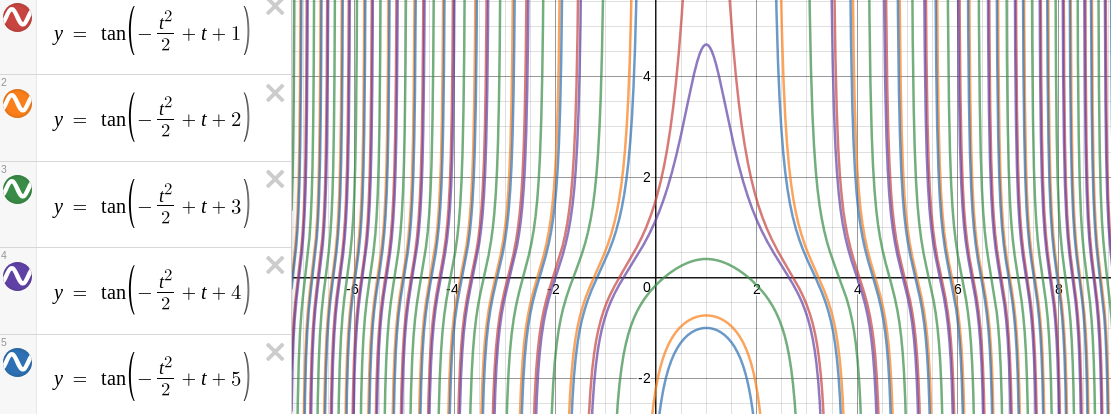
\includegraphics[width=15cm]{1d.png}
                    
                }

                % e)
                \item {
                    $ye^{xy}\cos{2x}-2e^{xy}\sin{2x}+2x+
                    (xe^{xy}\cos{2x}-3)\dv{y}{x}=0$

                    \color{azul}
                    % Respuesta
                    Consideremos $M = ye^{xy}\cos{2x}-2e^{xy}\sin{2x}+2x$ y $N =
                    xe^{xy}\cos{2x}-3$. \\[.3cm]
                    
                    Entonces
                    \begin{align*}
                        \dv{M}{y}
                        &= \dv{(ye^{xy}\cos{2x}-2e^{xy}\sin{2x}+2x)}{y}
                        = \dv{ye^{xy}}{y}\cos{2x} - 2\dv{e^{xy}}{y}\sin{2x} + 0 \\[.3cm]
                        &= (e^{xy} + xye^{xy}) \cos{2x}- 2xye^{xy}\sin{2x} \\[.3cm]
                        &= e^{xy}\cos{2x} + xye^{xy}\cos{2x} - 2xye^{xy}\sin{2x}
                    \end{align*}
                    
                    Y
                    
                    \begin{align*}
                        \dv{N}{x}
                        &= \dv{(xe^{xy}\cos{2x}-3)}{x} = \dv{xe^{xy}\cos{2x}}{x}
                        -\dv{3}{x} \\[.3cm]
                        &= e^{xy}\cos{2x} + x (ye^{xy}\cos{2x}
                        + e^{xy}(-\sin{2x})2) + 0 \\[.3cm]
                        &= e^{xy}\cos{2x} + x(ye^{xy}\cos{2x} - 2ye^{xy}\sin{2x})\\[.3cm]
                        &= e^{xy}\cos{2x} + xye^{xy}\cos{2x} - 2xye^{xy}\sin{2x}\\[.3cm]
                        &= \dv{M}{y}
                    \end{align*}
                    
                    Por lo que la ecuación es exacta. Esto es, que existe una
                    $\phi(x, y)$ tal que $\dv{\phi}{x} = M$ y $\dv{\phi}{y} = N$\\[.3cm]
                    
                    Para encontrar la primitiva, es más sencillo integrar $N$
                    respecto a $y$.
                    \begin{align*}
                        \phi(x, y) &= \int{N dy}
                        = \int{(xe^{xy}\cos{2x}-3) dy} \\[.3cm]
                        &= \cos{2x} \int{xe^{xy} dy} - \int{3dy}
                        = e^{xy}\cos{2x} - 3y + g(x)
                    \end{align*}
                    
                    Y queda como incógnita $g(x)$, pero se puede obtener usando
                    el hecho de que $M$ es la derivada respecto a $x$ de la
                    primitiva\\[.3cm]
                    
                    \begin{align*}
                        M = \dv{\phi(x, y)}{x}
                        &= \dv{(e^{xy}\cos{2x} - 3y + g(x))}{x} \\[.3cm]
                        ye^{xy}\cos{2x} - 2e^{xy}\sen{2x} + 2x
                        &= ye^{xy}\cos{2x} - 2e^{xy}\sen{2x} + g'(x)\\[.3cm]
                        \implies g'(x) = 2x &\implies g(x) = \int{2xdx} = x^{2}
                    \end{align*}
                    Por lo que la primitiva sin incógnitas es
                    \[\phi(x, y) = e^{xy}\cos{2x} - 3y + x^2 + C\]
                    Luego, despejando $y$.
                    \begin{align*}
                        \implies e^{xy}\cos{2x} &= 3y - x^2 - C\\[.3cm]
                        \implies e^{xy} &= \frac{3y - x^2 - C}{\cos{2x}} \\[.3cm]
                        \implies xy &= ln(\frac{3y - x^2 - C}{\cos{2x}}) \\[.3cm]
                        \implies y &= \frac{1}{x}ln(\frac{3y - x^2 - C}{\cos{2x}}) 
                    \end{align*}
                    Vemos que y no se puede despejar, pero se pueden aproximar las
                    soluciones con métodos de aproximaciones numéricas.\\[8cm]
                    
                    
                }

                % f)
                \item {
                    $(t+2)\sin{y}+t\cos{y}\dv{y}{t}=0$

                    \color{azul}
                    % Respuesta
                    Modificando la ecuación, tenemos que
                    \begin{align*}
                        &\implies t\cos{y}\dv{y}{t} = -(t+2)\sin{y} \\[.3cm]
                        &\implies \dv{y}{t} = -\frac{(t+2)\sin{y}}{t\cos{y}} \\[.3cm]
                        &\implies \dv{y}{t} = -\frac{\frac{t+2}{t}}{\cot{y}}
                    \end{align*}
                    Que es de la forma de una ecuación separable.\\[.3cm]

                    Por lo que,para resolverla, hay que resolver

                    \begin{align*}
                        &\implies \cot{y} dy = -(1 + \frac{2}{t})dt \\[.3cm]
                        &\implies \int{\cot{y} dy} = -\int{(1 + \frac{2}{t})dt} \\[.3cm]
                        &\implies ln \abs{\sin{y}}= -(t + 2 ln \abs{t}) + C \\[.3cm]
                        &\implies \abs{\sin{y}} =  e^{-(t + 2 ln \abs{t}) + C} \\[.3cm]
                        &\implies \sin{y} = ( e^{-(t + 2 ln \abs{t}) + C}) \\[.3cm]
                        &\implies y = \arcsin (e^{-(t + 2 ln \abs{t}) +C})\\[.3cm]
                        &\implies y = \arcsin (\frac{e^{-t-c}}{t^2})
                    \end{align*}
                    
                    De ahí, $y = \arcsin (\frac{e^{-t-c}}{t^2})$\\[4cm]
                    
                    
                }

                % g)
                \item {
                    $\left(3t+\frac{6}{y}\right)
                    +\left(\frac{t^2}{y}+3\frac{y}{t}\right)\dv{y}{t}=0$

                    \color{azul}
                    % Respuesta
                    Primero, hay que multiplicar todo por $ty$.
                    \[(3t^{2}y+6t)+(t^{3}+3y^{2})\dv{y}{t}=0\]
                    Entonces, con $M = 3t^{2}y+6t$ y $N = t^{3}+3y^{2}$ se tiene
                    que
                    \[\dv{M}{y} = 3t^{2} = \dv{N}{t}\]
                    Por lo que la ecuación es exacta, esto es que existe una
                    $\phi$ primitiva de $M$ y $N$\\[.3cm]
                    Luego, integrando $M$ respecto a $t$.
                    \[\int{M dt} = \int{(3t^{2}y+6t)dt} = t^{3}y + 3t^{2} + g(y)\]
                    Integrando $N$ respecto a $y$.
                    \[\int{N dy} = \int{(t^{3}+3y^{2})dt} = t^{3}y + y^{3} + h(t)\]
                    Por lo que la forma de la expresión sin incógnitas es
                    \[\phi(y, t) = t^{3}y + y^{3} + 3t^{2}\]
                    Luego, despejando $y$
                    \begin{align*}
                        &\implies y = -\frac{y^{3} + 3t^{2}}{t^{3}} \\[.3cm]
                        &\implies y + \frac{y^{3}}{t^{3}} = \frac{3}{t} \\[.3cm]
                        &\implies y + \frac{y^{3}}{t^{3}} - \frac{3}{t}  = 0 \\[.3cm]
                        &\implies y^{3} + yt^{3} - 3t^{2}  = 0
                    \end{align*}
                    Que está en la forma de una ecuación cúbica deprimida que,
                    por la fórmula de Cardano, tiene solución real
                    \begin{align*}
                        y &= \sqrt[3]{-\frac{-3t^{2}}{2} + \sqrt{\frac{(-3t^{2})^{2}}{4}
                    + \frac{(t^{3})^{3}}{27}}} + \sqrt[3]{-\frac{-3t^{2}}{2} - \sqrt{\frac{(-3t^{2})^{2}}{4}
                    + \frac{(t^{3})^{3}}{27}}} \\[.3cm]
                    &= \sqrt[3]{\frac{3t^{2}}{2} + \sqrt{\frac{9t^{4}}{4}
                    + \frac{t^{9}}{27}}} + \sqrt[3]{\frac{3t^{2}}{2} - \sqrt{\frac{9t^{4}}{4}
                    + \frac{t^{9}}{27}}}
                    \end{align*}
                }
            \end{enumerate}
        }


        % Ejercicio 2
        \pagebreak
        \item {
        	Hallar todas las funciones $g(t)$ que hacen que la ecuación
        	diferencial $$y^2\sen{t}+yg(t)\dv{y}{t}=0$$ sea exacta.

        	\color{azul}
        	Supongamos que la ecuación dada es exacta.

        	Sea $M(t,y)=y^2\sen{t}$ y sea $N(t,y)=yg(t)$. Como la ecuación
        	diferencial es exacta, entonces se cumple que
        	$\pdv{M}{y}=\pdv{N}{t}$, es decir
        	$$\pdv{M}{y}=2y\sen{t}=yg'(t)=\pdv{N}{t}$$
        	Entonces
        	$$g'(t)=2\sen{t}$$
        	$$g(t)=\int{2\sen{t}\dd t}=-2\cos{t}+h(y)$$
        	Para que la ecuación diferencial pueda resolverse es necesario que
        	la función $g$ sólo dependa de una variable, ya estaba establecida
        	la dependencia con la variable $t$, por lo que $h(y)=C$.

        	Por lo que la familia de funciones $g(t)=-2\cos{t}+C$ hacen que la
        	ecuación diferencial sea exacta.
        }

        % Ejercicio 3
        \pagebreak
        \item {
        	Las ecuaciones diferenciales de la forma $$\dv{y}{t}=f(y/t)$$ se
        	pueden resolver si se hace el cambio de variable $v=y/t$. Mostrar
        	que la ecuación toma la forma $$t\dv{v}{t}+v=f(v).$$ Usar este
        	método para resolver $$\dv{y}{t}=\frac{t+y}{t-y}.$$

        	\color{azul}
        	Sea $v=y/t$, entonces $y=vt$ y podemos hacer un cambio de variable
        	\begin{align*}
        	\dv{y}{t}             &= f(y/t)\\[.3cm]
        	\dv{(vt)}{t}          &= f(v)\\[.3cm]
        	v\dv{t}{t}+t\dv{v}{t} &= f(v)\\[.3cm]
        	t\dv{v}{t}+v          &= f(v)
        	\end{align*}
        	Ahora, para resolver la ecuación $\dv{y}{t}=\frac{t+y}{t-y}$
        	hacemos el cambio de variable $v=y/t$, o bien, $y=vt$.
        	\begin{align*}
        	\dv{(vt)}{t}          &= \frac{1+vt}{1-vt}\\[.3cm]
        	v\dv{t}{t}+t\dv{v}{t} &= \frac{t(1+v)}{t(1-v)}\\[.3cm]
        	v+tv'                 &= \frac{1+v}{1-v}\\[.3cm]
        	tv'                   &= \frac{1+v}{1-v}-v\\[.3cm]
        	tv'                   &= \frac{1+v^2}{1-v}\\[.3cm]
        	\frac{1-v}{1+v^2}v'   &= \frac{1}{t}
        	\end{align*}
        	Sea $F(v)$ tal que $F'(v)=\frac{1-v}{1+v^2}$ entonces $\dv{F(v(t))}
        	{t}=\dv{F}{v}\dv{v}{t}=\frac{1-v}{1+v^2}v'$, integramos respecto de
        	$t$ de ambos lados
        	\begin{align*}
        	\int{\dv{F(v)}{t}\,\dd t} &= \int{\frac{1}{t}\,\dd t}\\[.3cm]
        	\int{\frac{1-v}{1+v^2}\,\dd v} &= \ln{\abs{t}}+C\\[.3cm]
        	\int{\frac{1}{1+v^2}\,\dd v}-\int{\frac{v}{1+v^2}\,\dd v}
        	&= \ln{\abs{t}}+C\\[.3cm]
        	\tan^{-1}{v}-\frac{1}{2}\ln{\abs{1+v^2}}&=\ln{\abs{t}}+C
        	\end{align*}
        	No es posible despejar a la $v$, por lo que sólo resta revertir el
        	cambio de variable
        	$$\tan^{-1}{\left(\frac{y}{t}\right)}
        	-\frac{1}{2}\ln{\abs{1+\left(\frac{y}{t}\right)^2}}
        	=\ln{\abs{t}}+C$$
        }

        % Ejercicio 4
        \pagebreak
        \item {
        	Una población crece de acuerdo a la ley logística, y tiene un
        	límite de $5\times 10^8$ individuos. Cuando la población es baja se
        	duplica cada 40 minutos. ¿Qué valor tendrá la población después de
        	dos horas si inicialmente era de \emph{a}) $10^8$ individuos y
        	\emph{b}) $10^9$
        	individuos?

        	\color{azul}
        	La ley logística nos dice que
        	\[
        	P(t)=\frac{P_0 a}{P_0 b+(a-P_0 b)e^{-a(t-t_0)}}
        	\]
        	donde $\frac{a}{b}=5\times 10^8$ marca el límite o estabilidad
        	poblacional, $P_0$ es la población inicial, $t_0$ es el tiempo
        	inicial (que en este caso lo consideraremos $t_0=0$).

        	Cuando la población es baja utilizamos la ecuación logística
        	$\dv{P}{t}=KP_0$ cuya solución es $P(t)=(P_0)e^{at}$. Utilizaremos
        	esta información para encontrar el valor de $a$ y eventualmente el
        	de $b$.
        	\begin{enumerate}
        		\item Si $P_0=10^8$ y sabemos que
        		$P(40)=2\times 10^8=10^8e^{a(40)}$. Despejando a la $a$
        		\begin{align*}
        		2 &= e^{40a}\\
        		\ln{2} &= 40a\\
        		a &= \frac{\ln{2}}{40}\\
        		a &\approx 0.01733
        		\end{align*}
        		Por el límite de población, tenemos que
        		$\frac{a}{b}=5\times 10^8$, ahora que tenemos $a$ podemos
        		encontrar $b$
        		\begin{align*}
        		b &= \frac{a}{5\times 10^8}\\[.2cm]
        		b &= \frac{\frac{\ln{2}}{40}}{5\times 10^8}\\[.2cm]
        		b &= \frac{\ln{2}}{200\times 10^8}\\[.2cm]
        		b &\approx 34.65\times 10^{-12}
        		\end{align*}
        		Ya que tenemos todo lo que necesitamos, podemos aplicar la
        		ecuación logística inicial, con el tiempo en minutos (para
        		simplificar la notación se han dejado los valores de $a$ y de
        		$b$ expresado con sus literales):
        		\begin{align*}
        		P(120) &= \frac{a\times 10^8}
        		{b\times 10^8+(a-b\times 10^8)e^{-a(120-0)}}\\[.3cm]
        		&\approx \frac{1732867.95}{0.003465+(0.01386)
        			e^{-0.01733(120)}}\\
        		&\approx 333'333'333.33\\
        		&\approx 3.3333\times 10^8 \text{ individuos.}
        		\end{align*}

        		\item Ahora si $P_0=10^9$ individuos procedemos de manera
        		análoga.
        		\begin{align*}
        		P(40)=2\times\cancel{10^9}&=\cancel{10^9}e^{a(40)}\\[.2cm]
        		2 &= e^{40a}
        		\end{align*}
        		Por lo que los valores de $a$ y de $b$ no dependen de la
        		población inicial y son los mismos que en inciso anterior.

        		Aplicando la ecuación logística
        		\begin{align*}
        		P(120) &= \frac{a\times 10^9}
        		{b\times 10^9+(a-b\times 10^9)e^{-a(120-0)}}\\[.3cm]
        		&\approx \frac{17328679.514}{0.03465+(-0.01732)
        			e^{-0.01733(120)}}\\[.3cm]
        		&\approx 533'333'333.33\\[.2cm]
        		&\approx 5.3333\times 10^8 \text{ individuos.}
        		\end{align*}
        		Notemos que en este caso la población supera el límite
        		poblacional que era de $5\times 10^8$, esto puede deberse a que
        		consideramos la población inicial de $10^9$ como ``baja''
        		cuando en realidad no hay un criterio adecuado para determinar
        		cuando la población es considerada como ``baja''. Sin embargo
        		al aplicar la ecuación logística para tiempos más grandes
        		podemos notar que la población se estabiliza hacia su límite,
        		por ejemplo $P(240)\approx5.04\times 10^8$ individuos.
        	\end{enumerate}
                }
    \end{enumerate}
\end{document}
